\chapter{Laboratorio:  Programación con LOGO!}
	  
\section{\obj}
Este  laboratorio busca:
\begin{itemize}
	{\small
    \item Programar e implementar un arranque en Estrella -Delta usando un el relé inteligente LOGO!.
    \item Programar e implementar un alternador de dos bombas.
    \item Programar un alternador de bombas con señales de alarma y temporizadores semanales.
    \item Aprender las conexiones eléctricas de las entradas y salidas del controlador.
    \item Calcular el ciclo de trabajo de cada programa de cada programa 
 }
\end{itemize} 

 
\section{Equipos y materiales}
Para este laboratorio de necesitaran:
\begin{itemize}
	{\small \item 2 motores trifásicos 1/2 hp de 3 puntas.
		\item 1 motor trifásico de 6 puntas.
	\item 1 Logo! 230RC de Siemmens.
	\item 1 Software LOGO! Confort.
	\item 4 contactores.
	\item 1 botón pulsar cerrado.
	\item 3 botones pulsadores abiertos.
	\item 1 \href{https://cache.industry.siemens.com/dl/files/041/109741041/att_924629/v1/logo_system_manual_es-ES_es-ES.pdf}{Manual del LOGO! 8}.
	\item 1 \href{https://cache.industry.siemens.com/dl/files/807/100782807/att_924633/v1/Help_es-ES_es-ES.pdf}{Manual LOGO!Soft Comfort.}
}
\end{itemize}

\section{Marco de referencia}

Como se indica en el manual \cite{LOGO1}, el LOGO! un módulo lógico universal para el control de procesos industriales o automatización, que incorpora funciones lógicas, temporizadores, contadores, controladores PID, funciones aritméticas, fuente de alimentación, interfaces gráficas, módulos de ampliación y el software de programación. La figura muestra un LOGO!8 24CE, de 24 voltios y salidas a transistor.
\begin{figure}
	\centering
	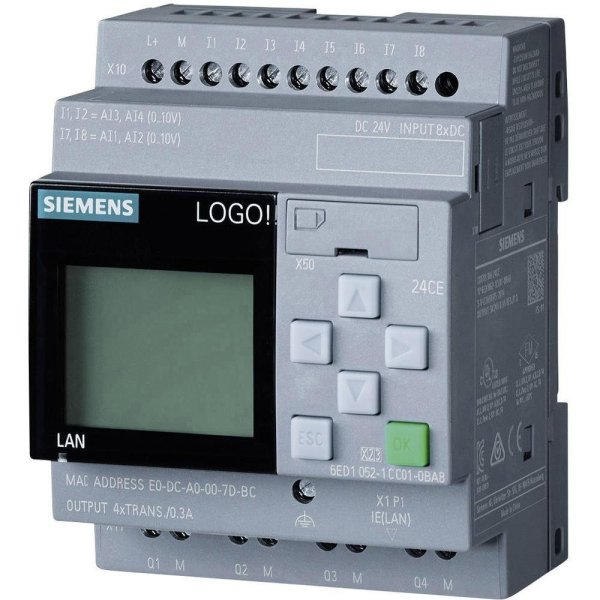
\includegraphics[width=0.5\linewidth]{fig/Logo!8.jpg}
	\caption{LOGO!8 24CE.}
	\label{fig:logo8}
\end{figure}

 El alambrado del dispositivo esta explicado en la sección 2.3 del Manual del LOGO! \cite{LOGO1}. Hay que tener en cuenta que dependiendo del modelo del LOGO, la forma de como se alambra la alimentación, las señales de entradas y las señales de salida podrían cambiar. Respecto a la alimentación, es importante la colocación de fusibles o varistores (MOV) dependiendo del modelo, ver pagina 43 del manual.  Un ejemplo básico de un programa de control en LOGO, con el alambrado físico se muestran en la sección 3.3 del manual \cite{LOGO1}.
 
 El LOGO es programado con el software llamado \href{https://new.siemens.com/global/en/products/automation/systems/industrial/plc/logo/logo-software.html}{\textit{LOGO!Soft Comfort}}. En el manual del software \cite{LOGO2}, en el capítulo 3, página 164, se muestra un Tutorial del uso del programa. Por otra parte, dicho manual brinda los siguientes cinco ejemplos resueltos para su estudio:
 
\begin{itemize}
	\item Bomba de agua no potable (página 219).
	\item Sistema de ventilación (página 235).
	\item Portón corredizo (página 236).
	\item Control de calefacción (página 238).
	\item Estación de llenado (página 241).	
\end{itemize}
 
 
\section{Metodología}

Este laboratorio tiene una duración de 4 lecciones, repartidas en dos semanas. Los estudiantes deben mostrar durante las clases programadas las tres actividades propuestas. Deben recabar fotografías y resultados de los equipos de medición para elaborar las evidencias. Las evidencias se subirán al TecDigital la semana siguiente finalizadas las actividades.

\section{Práctica en Clase}

\subsection{Actividad 1}

	El profesor realizara el programa de control para un arranque en estrella-delta en LOGO!Soft Comfort y explicará todo lo concerniente a: simulación del programa, y a la configuración de la red local (LAN), Mascara, pasarela de salida (gateway), y carga en el programa. 
	
 \subsubsection{Conteste las preguntas}
 	¿Que información brinda el comando IPCONFIG en COMMAND PROMPT de Windows?, ¿Que información brinda el comando PING?.  

\subsection{Actividad 2}


Diseñe el programa para el controlador LOGO!, que resuelva el siguiente problema.

Se necesita un alternador de bombas  para el llenado de un tanque de almacenamiento. El taque posee tres niveles, NA nivel alto, NB nivel bajo y Nivel Crítico NC, además existen 2 bombas B1 y B2. Cuando el agua activa NB la bomba B1 se activa y se apaga hasta alcanzar el nivel NA. La próxima vez que se active el sensor NB se activa la segunda bomba B2 y se apaga hasta alcanzar NA. Este ciclo se repite hasta que se presione el apagado general del sistema o se active una de las dos sobrecargas. Si el nivel crítico se presiona NC se encienden ambas bombas, además el sistema debe  recordar el orden de la alternancia. El sistema cuenta con dos botoneras para el arranque y pare general del sistema. El sistema deberá mostrar en pantalla en todo momento,  el estado de la bombas y la etapa lógica en que se encuentra el sistema.

Una vez simulada la solución, procederá a cargarla y alambrar el LOGO!. Para esto requerirá de las botoneras pulsadoras, contactores y finales de carrera que emulan los niveles de la boyas, etc. 

% \begin{figure}
%     \centering
%     \begin{circuitikz}
%     \draw (0,0)
%     to [esource, l=$F$] --++ (1,0) 
%     ;
%     \end{circuitikz}
%     \caption{Caption}
%     \label{fig:enter-label}
% \end{figure}


\subsubsection{Conteste las preguntas}

¿Puede mostrar el diagrama lógico de la solución?, ¿Puede mostrar el diagrama de la implementación con sus  ecuaciones lógicas?, ¿Puede mostar el diagrama de conexión eléctrico?.¿Cuando es el ciclo de escaneo de la solución? La ultima pregunta se contesta implementando el código que se aporta en apéndice B del manual \cite{LOGO1}.

\subsection{Actividad 3}
Diseñe el programa para el controlador LOGO!, que resuelva el siguiente problema.

La empresa \textbf{Automation Solutions} necesita controlar dos moto-bombas de forma alternada.

Las entradas del sistema son:  botón del arranque motor A, botón de paro del motor A,  presostato de confirmación del motor A, botón del arranque motor B, botón de paro del motor B,  presostato de confirmación del motor B. 

Las salidas del controlador son las señales a los contactares de la moto-bomba A y la moto-bomba B.

El sistema debe funcionar con la siguiente lógica:

\begin{itemize}
	\item Si el sistema esta en modo manual, el arranque y pare se realiza desde las botoneras. Si a los 3 segundos no existe la señal de confirmación de presión, aparece en pantalla del LOGO! un mensaje indicando que la bomba no levanta presión, y se desactiva el enclave-miento de  la señal del motor.
	\item Por otra parte, si la maneta esta en la posición de modo automático, la bomba X se enciende a las 5PM y se apaga a las 10PM. El arranque y pare de las moto-bombas es de forma alternada. Es decir, si el Lunes arranca la  moto-bomba B1, el Martes deberá arrancar la moto-bomba B2 y así sucesivamente. Si la confirmación de presión no se recibe en un lapso de 3 segundo, el sistema cambiará a la otra bomba y mostrara en pantalla el aviso del cambio.	
	\item Adicionalmente, existe un  contador que indica en pantalla del LOGO!, la cantidad de ciclos de la bomba 1 y de la bomba 2. Cuando los ciclos realizados sean igual a 10 aparecerá en pantalla un mensaje indicando : “La bomba Bx requiere mantenimiento”. En pantalla se debe indicar la etapa lógica del sistema.
\end{itemize} 




\subsubsection{Conteste las preguntas}
¿Puede mostrar el diagrama lógico de la solución?, ¿Puede mostrar el diagrama de la implementación con sus  ecuaciones lógicas?, ¿Puede mostar el diagrama de conexión eléctrico?.¿Cuando es el ciclo de escaneo de la solución? La ultima pregunta se contesta implementando el código que se aporta en apéndice B del manual \cite{LOGO1}.



